\chapter{螺旋线} \label{ch3}
慢波系统是行波管的主要部件之一,它是管内传播高频电磁波的一种特殊传输线。按照在行波管中所起的作用,我们对慢波线提出了以下三个基本要求:一是能使高频电磁波的传播速度减慢,以便与电子流“同步”,进行充分的能量交换;二是要求慢电磁波的传播速度随频率的变化尽量小,这样,当不同频率的电磁波进入该慢波线时就都能与电子流“同步”,因而都能得到放大,行波管的频带就能做得很宽。讲到这里,读者也许要问:在第二章里不是说过传输线的频带是很宽吗?这里为什么又作为一条基本要求提出来呢?这是因为慢波线一般都不是均匀的传输线,我们知道,均匀传输线(如同轴电缆)的频带是非常宽的,而非均匀传输线的频带就要窄得多,非均匀传输线的频带宽度是与它们的不均匀程度有密切的关系的,不同的慢波线,由于其结构上的不同就会带来频带宽度的不同。因此,我们在设计慢波线的时候,很重要的一点就是要算出它的频带宽度是否能满足我们的要求。对于慢波线的第三个基本要求是希望在慢波线中电子注通过的地方能够建立起较强的轴向电场,这样,电子与高频电场之间才能产生有效的能量交换。

上一章中提到的螺旋线是一种能够较全面地满足上面三个基本要求的慢波线。特别是由于它具备了频带宽这样一条突出的优点,加上其结构简单、容易制作,所以中小功率行波管中几乎毫无例外地都采用螺旋线来作为它们的慢波系统。本章将对螺旋线的主要特效及若干实际问题作一简略介绍。
\section{螺旋线是怎样使电磁波速度变慢的?}
我们来看看图\ref{ch3-1}所示的一根用细金属丝绕成的螺旋线假定它的轴线与坐标轴$ Z $轴重合,平均直径等于$ 2a $,螺距等于$ p $,螺旋角(螺旋线上任意一点的切线与过该点所作$ Z $轴垂直平面之间的夹角称为螺旋角)等于$ \psi $。当电磁波以光速$ c $从螺旋线上的某点$ A $沿细金属丝传播到另一点$ B $时,如果$ B $点正好是沿金属丝绕行一圈到达的那个点,那么,电磁波沿金属丝所传播的距离可由图\ref{ch3-1}右边所示的一圈螺旋线的展开图上求得,它等于$\frac{2\pi a}{\cos \psi} $。但如果我们来观察同一时间内电磁波沿$ Z $轴的传播距离的话,它只前进了一个螺距$ p $。因此,电磁波沿$ Z $轴的传播速度$ v_p $与光速$ c $的比值等于:
\begin{equation}
	\frac{v_p}{c} = \frac{p}{\frac{2\pi a}{\cos \psi}} = \frac{p}{2\pi a}\cdot \cos\psi
\end{equation}
它反映了电磁波沿$ Z $轴的传播速度比光速减慢的程度,叫做螺旋线的“慢波比”。如果知道了电子注的运动速度$ v_0 $,那么就可以适当选择螺旋线的几何尺寸,使得$ v_p \approx v_0 $,即实现电磁波与电子注的“同步”。如前所述,在行波管实际工作时,为了达到真正的“同步”,通常还需要用改变螺旋线电压的办法来调节$ v_0 $,也就是进行“细调”。
\begin{figure}[phtb]
	\centering
	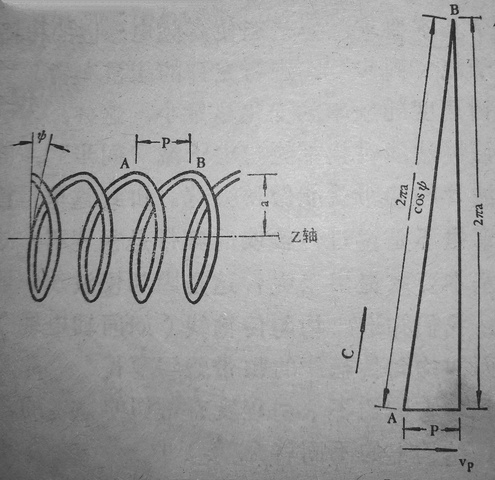
\includegraphics[width=0.65\linewidth]{figure/ch3-1}
	\caption{螺旋线的螺距、螺旋角和半径:$ \frac{v_p}{c} = \frac{p}{2\pi a} \cos \psi$}
	\label{ch3-1}
\end{figure}

上面的分析方法虽然便于直观地理解螺旋线中电磁波传播速度变慢的工作原理,但是,应该指出,这种分析是很粗略的。因此,它不能十分准确地反映实际情况。比如,由它似乎可以得出“慢电磁波的传播速度不随频率而变化”[因为式\ref{ch3-1}中不包含频率$ f $这样的错误结论。实践证明,对一个结构一定的螺旋线来说,虽然慢电磁波的传播速度在一定的频率范围内变化较小,但毕竟还是有变化的,这种变化对于行波管的工作是有影响的。因此,为了准确地设计螺旋线的结构,保证行波管的宽频带运用,就必须进一步研究慢电磁波的传播速度与频率之间的关系,即“色散特性”。


\section{色散特性}
慢电磁波的传播速度随频率而变化的情况,通常都用慢波系统的色散特性来表示。“色散”原是指光学中的一个物理现象。我们知道,光也是一种电磁波,只是它的频率要比微波高得多罢了。光因其频率的不同而呈现各种颜色,而白光则是由多种频率的单色光混合而成的。不同颜色的光在真空中传播时速度都是相同的,但是在介质(例如玻璃等)中传播时,它们的速度就随频率而不同了。因此,如果让不同颜色的光以同一个方向从空气中斜入射到玻璃介质中去,那么,由于折射角将随频率而变化,它们在玻璃中的传播方向就各不相同了。我们可以做一个实验来证实这个现象:让一束白光从空气中入射到玻璃棱镜中去,在玻璃棱镜的后面放置一个白色的屏幕,那么,白光中的各种单色光就将以不同的折射角从玻璃棱镜中射到白色屏幕上,于是,在白色屏幕上我们就可以看到依次排列的红、橙、黄、绿、青、兰、紫等各种颜色,这种现象便称为色散”。可见,色散的本质就是光在介质中的传播速度随频率而变化的特性。我们在描述慢波线中慢电磁波的传播速度随频率而变化的特性时,也采用了这个名称。

螺旋线的色散特性可以通过理论分析和实验测量两种途径得到。图\ref{ch3-2}所表示的螺旋线色散特性,就是在对实际螺旋线作了一定简化假设的条件下,用电磁场理论对电磁波沿螺旋线的传播规律进行数学分析后得出来的。图中纵坐标为$ \frac{v_p}{c} $,因为光速$ c $为常数,所以纵坐标的值是与$ v_p $正比的。横坐标为$ ka $其中$ a $是螺旋线的平均半径,对于结构已经确定的螺旋线来说,$ a $是一个常数。$ k=\frac{2\pi f}{c} $是电磁波在自由空间传播时的相位传播常数,它的物理意义将在后面介绍。由上可见,横坐标$ ka $是与频率$ f $成正比的。因此,图\ref{ch3-2}就表示了$ v_p $和$ f $的关系,也就是色散特性。
\begin{figure}[phtb]
	\centering
	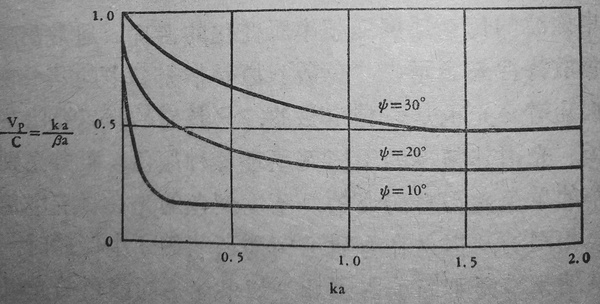
\includegraphics[width=0.65\linewidth]{figure/ch3-2}
	\caption{螺旋线的色散特性曲线}
	\label{ch3-2}
\end{figure}

从图\ref{ch3-2}的曲线中我们可以看到,当频率较高时,$ v_p $基本不变,且只与螺旋角$ \psi $有关。它的数值可以近似用$ \ref{ch3-1} $式算得,在$ \psi $较小的情况下,$ \ref{ch3-1} $式可以写成:
\begin{equation} \label{eq:ch3-2}
	\frac{v_p}{c}= \sin \psi \approx \tan\psi = \frac{p}{2\pi a}
\end{equation}
可以看出,\ref{eq:ch3-2}式是与上一章中的\ref{eq:ch2.1}式一致的。在实际的行波管中,工作频率不能任意提高,因为当频率超过一定范围后将会引起返波振荡(见第\ref{ch5}章),造成行波管工作的不稳定。为了避免返波振荡出现,通常在设计螺旋线时,总是使$ ka < 0.3 $。

我们在设计螺旋线型行波管时,常常是根据一定的原则先确定电子注电压(即螺旋线电压)$ U_0 $,从而也就决定了电子速度$ v_0 $和慢电磁波的传播速度$ v_p $。例如,微波通信设备所用的某中小功率行波管,其$ U_0 $为3千伏,对应的电子速度$ v_0 $约为光速$ c $的十分之一,由此可算得螺旋角约$ 6^\circ $。由图\ref{ch3-2}可见此时的色散特性曲线上有很宽的弱色散区(弱色散区是指$ v_p $随$ f $变化很小的区域,角越小,弱色散区越宽)。因此,尽管把$ ka $限制在0.3以下,由于$ U_0 $较低,$ \psi $较小,我们仍然可以得到很宽的频带。例如,对上例中$ \psi \approx 6 ^\circ $的情况,$ ka $只要大于$ 0.1 $左右,特性就很平了,如果$ a=1.5 $毫米,那么与$ 0.1<ka<0.3 $相对应的频率范围就是$ 3.2<f<9.5 $千兆赫,可见频带是很宽的。

慢波线的色散特性除了能够用$ \frac{v_p}{c}\textasciitilde ka$曲线直观地表示以外,还可以用所谓“$\omega -\beta $”曲线来表示,而且$ \omega-\beta $曲线能够更多地反映出慢波系统的主要特性。为了说明这个曲线,我们先来熟悉一下描述电磁波传播特性的几个基本量。

假设电磁波沿慢波线的轴线($ Z $轴)方向向前传播,电磁波的频率为$ f $,如果略去慢波线的损耗,那么,其高频电场和磁场都是一个随时间$ t $和距离$ Z $按正弦规律作周期性变化的等幅波。通常我们只考虑轴向高频电场分量$ \tilde{E_z} $,因为与电子流产生能量交换的,主要就是轴向电场分量。$ \tilde{E_z} $随时间和空间距离的变化可以用下面的数学公式来描述:
\begin{equation} \label{eq:ch3-3}
	\tilde{E_z} = \hat{E_z}\sin(wt-\beta Z)
\end{equation}
式中$ \hat{E_z} $为高频电场的幅度。$ (wt-\beta Z) $为$ \tilde{E_z} $的相位角。由正弦函数的周期性可知,相位角$ (wt-\beta Z) $每改变$ 2\pi $弧度,$ \tilde{E_z} $的变化将完成一次循环而等于原来的值,我们称这些点为同相位点。

\eqref{eq:ch3-3}式表明,高频电场$ \tilde{E_z} $随时间$ t $和空间距离$ Z $都是正弦变化的。如果我们想在任意一点$ Z=Z_0 $处观察高频电场的变化,那么就可以把$ Z=Z_0 $代入\eqref{eq:ch3-3}式,于是得:
\begin{equation} \label{eq:ch3-4}
	\tilde{E_z} = \hat{E_z}\sin(wt-\beta Z_0)
\end{equation}
当$ Z_0=0 $时,\ref{eq:ch3-4}可简化成:
\begin{equation} \label{eq:ch3-5}
\tilde{E_z} = \hat{E_z}\sin{wt}
\end{equation}
因此,在任意一点看,高频电场都是随时间作正弦变化的。式中$ \omega $称为角频率,它表示单位时间内相位角的变化。高频电场变化一个循环(或称变化一周)所需的时间叫做周期$ T $。周期$ T $和频率$ f $之间有下列关系:
\begin{equation} \label{eq:ch3-6}
	T = \frac{1}{f}
\end{equation}
它的物理意义是很清楚的。在一个周期内相位角$ \omega t $的变化应为$ 2\pi $弧度,即$ \omega T = 2\pi $,把\eqref{eq:ch3-6}式代入,则得:
\begin{equation} \label{eq:ch3-7}
	\omega = \frac{2\pi}{T} = 2\pi f
\end{equation}
 
 同样,如果我们在任意一个时刻$ t=t_0 $观察整个空间高频电场的分布的话,那么可以看到$ \tilde{E_z} $随空间距离$ Z $也是正弦变化的。此时,\eqref{eq:ch3-3}式变为:
\begin{equation} \label{eq:ch3-8}
	\tilde{E_z} = \hat{E_z}\sin(\omega t_0 - \beta Z)
\end{equation}
若$ t_0 = 0 $,则上式可简化为:
\begin{equation} \label{eq:ch3-9}
\tilde{E_z} = \hat{E_z}\sin(- \beta Z)
\end{equation}
 式中$ \beta $称为轴向相位传播常数,或简称相位常数,它表示单位距离内相位角的变化。$ \tilde{E_z} $在空间变化一个周期所经过的距离叫做导波波长,用$ \lambda_g $表示。一个导波波长内相位角的变化也是$ 2\pi $,即$ \beta \cdot \lambda_g = 2\pi $,故得:
 \begin{equation} \label{eq:ch3-10}
 	\beta = \frac{2\pi}{\lambda_g}
 \end{equation}

下面,我们来看看电磁波的传播速度$ v_p $应该如何计算。由\eqref{eq:ch3-8}式可以作出不同的$ t_0 $下$ \tilde{E_z} $随$ Z $的变化曲线,我们发现每经过一个周期$ T $,则同相位点就沿$ Z $轴向前移动一个导波波长$ \lambda_g $的距离。例如在图\ref{ch3-3}中,我们画出了$ t=0 $和$ t=\frac{1}{4}T $两个时刻下的$ \tilde{E_z} $空间变化曲线,可以看出,同相位点(如$ A $与$ A' $,$ B $与$ B' $等等)之间的距离正好等于$ \frac{1}{4} \lambda_g$。因此,整个高频电场的正弦波形沿$ Z $轴的移动速度$ v_p $就等于:
\begin{equation} \label{eq:ch3-11}
	v_p = \frac{\lambda_g}{T}
\end{equation}
可见,所谓慢电磁波的传播速度$ v_p $实际上就是同相位点的移动速度,故$ v_p $常称为相速。

 \begin{figure}[phtb]
	\centering
	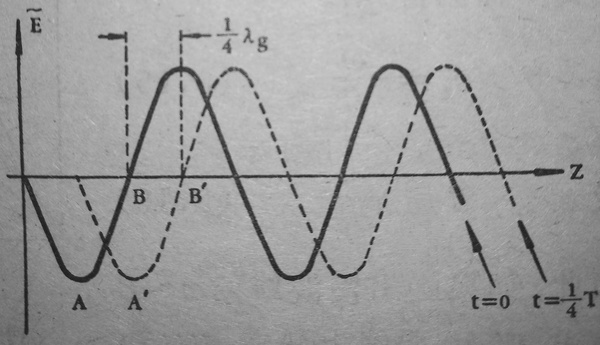
\includegraphics[width=0.5\linewidth]{figure/ch3-3}
	\caption{$ t=0 $和$ t=\frac{1}{4}$时刻,场分量沿$ Z $轴的变化曲线}
	\label{ch3-3}
\end{figure}

\eqref{eq:ch3-11}式可化为:
\begin{equation} \label{eq:ch3-12}
	\lambda_g = v_p \cdot T = \frac{v_p}{f}
\end{equation}

我们知道,在自由空间中,电磁波的波长$ \lambda_0 $与频率$ f $之间满足下面的关系:
\begin{equation} \label{eq:ch3-13}
	\lambda_0 = \frac{c}{f}
\end{equation}
由\eqref{eq:ch3-12}式和\eqref{eq:ch3-13}式可得:
\begin{equation} \label{eq:ch3-14}
	\frac{\lambda_g}{\lambda_0} = \frac{v_p}{c}
\end{equation}
可见,慢波线中的导波长$ \lambda_g $小于自由空间波长$ \lambda_0 $,二者之比即等于慢波比。例如,前面所举的例子中$\frac{v_p}{c}  \approx 0.1$,因此$ \frac{\lambda_g}{\lambda_0} = 0.1$,若$ \lambda_0 = 7.5 $厘米则$ \lambda_g=0.5 $毫米。 由\eqref{eq:ch3-7}、\eqref{eq:ch3-10}和\eqref{ch3-11}三式,我们得到:
\begin{equation} \label{eq:ch3-15}
	v_p =\frac{\omega}{\beta}
\end{equation}及
\begin{equation}\label{eq:ch3-16}
	 \beta = \frac{\omega}{v_p}
\end{equation}
 因此,如果画出慢波线的$ \omega \textasciitilde \beta $曲线,那么,曲线上任意一点和原点连线的斜率$ \frac{\omega}{\beta} $就是该点的相速$ v_p $。图\ref{ch3-4}是螺旋线的$ \omega \textasciitilde \beta $曲线。
 
 \begin{figure}[phtb]
 	\centering
 	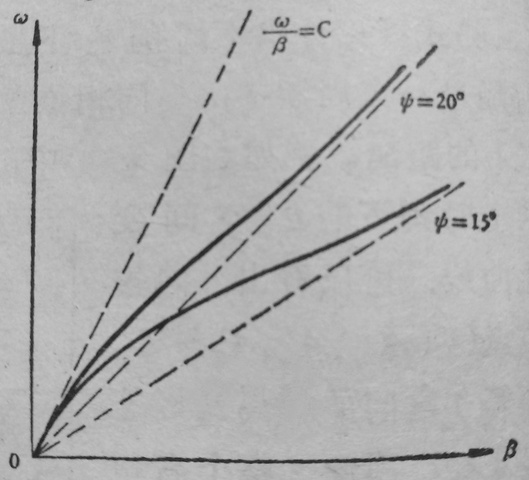
\includegraphics[width=0.42\linewidth]{figure/ch3-4}
 	\caption{螺旋线的$ \omega \textasciitilde \beta $曲线}
 	\label{ch3-4}
 \end{figure}
 
 顺便指出一点,如果比较一下\eqref{eq:ch3-16}和前面提到的$ k = \frac{2\pi f}{c} = \frac{w}{c} $,我们就可以明白为什么把$ k $称为自由空间中的相位传播常数了。
 
 由$ \omega - \beta $曲线我们还可以确定慢波线的一些其它传播特性。例如曲线上任意一点的切线斜率就等于波的“群速”$ v_g $(即波的能量传播速度,它和波的相位传播速$ v_p $不同);由曲线的形状可以判断出$ v_g $和$ v_p $的符号是否相同,实际上就是群速和相速的方向是否相同?我们把$ v_g $和$ v_p $,方向相同的波称为“前向波”,而$ v_g $和$ v_p $方向相反的波则称为“返波”。正是由于$ \omega - \beta $曲线能够更多地表示出慢波线的传播特性,所以应用更为广泛。

关于波的群速、前向波与返波等问题,因超出了本书范围,这里不赘述。
\section{耦合阻抗}
耦合阻抗是表征慢波线中轴向高频电场与电子之间能量交换的有效程度的一个参量(用符号$ K_c $表示)。在螺旋线型行波管中,电子注是在螺旋线内沿着它的轴线方向运动的,因此,只有轴向高频电场才能和电子产生能量交换作用。当电磁波沿螺旋线向前传播时,它在电子注流过处(具体说来也就是螺旋线内半径为$ b $的细圆柱体内。$ b $是电子注半径)产生的轴向高频电场越强,那么电子与轴向高频电场的能量交换作用也越强。电子注流过处轴向高频电场的大小与螺旋线的结构有关,螺旋线结构不同时,它的高频场分布就不同,因此为了求出电子注流过处轴向高频电场的大小,就需要找到螺旋线的场分布,图\ref{ch3-5}表示了螺旋线周围的高频场分布。

\begin{figure}[phtb]
	\centering
	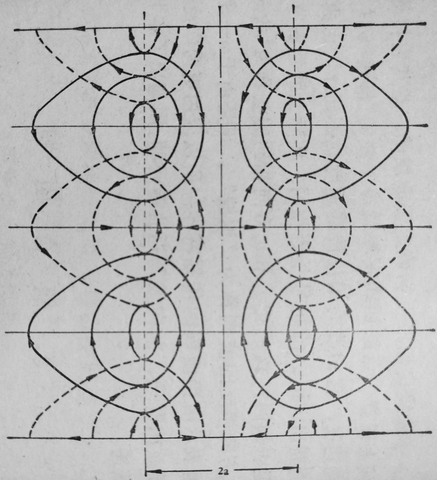
\includegraphics[width=0.55\linewidth,angle=90]{figure/ch3-5}
	\caption{螺旋线周围电场和磁场分布示意图。实线为电力线,虚线为磁力线。}
	\label{ch3-5}
\end{figure}

电子注流过处轴向高频电场的大小还与螺旋线中传播的高频场功率有关。显而易见,送入螺旋线的高频场功率越大,那么它在电子注流过处产生的轴向高频电场也越强。为了便于对不同的螺旋线中电子与场能量交换的有效程度进行比较,我们希望能建立一个统一的衡量标准。首先,在不同的螺旋线中应该送入相同的高频场功率。在相同的高频场功率下,我们再来观察哪一种螺旋线所产生的轴向高频电场大,这样才能比较出哪一种螺旋线的相互作用有效程度强。这实际上就是希望在新导出的用来衡量相互作用有效程度的参量中去掉高频场功率带来的影响。从$\text{压强}= \frac{\text{压力}}{\text{受压面积}} $(即压强等于单位面积所受到的压力)这个公式我们联想到,这个新参量是否可以用送入单位功率所产生的轴向高频电场的大小来表示呢?根据这个想法并类比了低频电路的情况,人们导出了一个新的参量,这就是耦合阻抗$ K_c $。

我们知道,在低频电路中,当我们在谐振频率下往某一谐振回路中送入一定的功率$ P $时,在回路两端所产生的谐振电压振幅$ U $和回路的谐振电阻$ R $有下面的关系:
\begin{equation} \label{eq:ch3-17}
	R = \frac{1}{2}\frac{U^2}{P}
\end{equation}
回路的谐振电阻$ R $越大,那么其两端产生的谐振电压也越大因此$ R $是表征谐振回路特性的一个重要参量。

同样道理,我们把慢波系统的耦合阻抗$ K_c $定义为:
\begin{equation} \label{eq:ch3-18}
	K_c = \frac{1}{2}\frac{\hat{U_z^2}}{P}
\end{equation}
式中$ P $为沿螺旋线传播的高频场总功率。$ \hat{U_z} $为轴向高频电压的振幅,它是从低频电路的关系式\ref{eq:ch3-17}中类比得来的。我们知道,在微波频率下,通常只采用高频电场这个概念,例如我们常常用场强计来测量高频电场的大小,用功率计来测量高频场的功率大小,而从不用伏特计(电压表)来测量微波高频电场。因此,这里所说的轴向高频电压$ \hat{U_z} $是为了和低频电路类比而人为地导出来的一个量,不过,我们可以利用直流电路中电压和电场之间的关系把它和轴向高频电场$ \hat{E_z} $联系起来。我们知道,在均匀直流电场中,$ a $、$ b $两点之间的电压$ U_{ab} $可用电场$ E $和两点之间的距离$ d_{ab} $表示:
\begin{equation} \label{eq:ch3-19}
	U_{ab} = -E\cdot d_{ab}
\end{equation}
负号表示$ U $和$ E $的方向相反。如果不是均匀电场,那么,可以用积分形式表示:
\begin{equation} \label{eq:ch3-20}
	U_{ab} = - \int_{a}^{b}E \cdot \text{d}z
\end{equation}
我们这里的轴向高频电场也不是均匀电场,不过它是一个有规律的非均匀电场,它是按照正弦规律变化的,如在某时刻$ t=0 $观察,则可简化成\ref{eq:ch3-9}式。为了方便起见,我们人为地取$ \tilde{E_Z} $由零变化到最大值这个四分之一周期所对应的轴向距离(即$\frac{1}{4}\lambda_g$)来作为积分区间,于是有:
\begin{equation} \label{eq:ch3-21}
	\hat{U_Z} = -\int_{0}^{\frac{\lambda_g}{4}}\tilde{E_z}\text{d}z=\int_{\frac{\lambda_g}{4}}^{0}\hat{E_z}\sin{\beta z}\text{d}z=\frac{\hat{E_z}}{\beta}
\end{equation}
读者可能要问:积分区间如果取二分之一导波波长行不行呢?回答是完全可以,但必须在任何场合下都这样规定,也就是说应当统一。

将\ref{eq:ch3-21}式代入\ref{eq:ch3-18}式,我们就可以得到耦合阻抗$ K_c $:
\begin{equation} \label{eq:ch3-22}
	K_c = \frac{\hat{E_z^2}}{2\beta^2P}
\end{equation}

由式\ref{eq:ch3-22}可见,流过慢波系统的功率流$ P $一定时,能够建立的轴向场强$ \hat{E_z} $愈强,则慢波系统的耦合阻抗也越大,也就能使场与电子的相互作用越强烈。而一定功率流下所能建立的电场的强弱主要决定于慢波系统的结构和尺寸,所以耦合阻抗$ K_c $的大小就表征了慢波系统在这方面质量的优劣。

知道了螺旋线内轴向电场分布以后,就可以计算出它的耦合阻抗。\ref{eq:ch3-9}式给出了场沿$ Z $轴方向的分布情况。但轴向电场在螺旋线横截面上是怎样分布的呢?图\ref{ch3-6}给出了它的理论分析结果。图中横坐标为螺旋线横截面内从中心出发沿半径方向的距离$ r $,纵坐标为$ r $处轴向电场$ E_z $与螺旋线上($ r=a $处)轴向电场$ E_{za} $的比值。由图可见,轴向电场在螺旋线横截面上不是均匀分布的,而是中心处最弱,半径$ a $处最强。所以计算所得的耦合阻抗$ K_c $沿径向的分布也有相似的曲线形状如图\ref{ch3-7}所示。由于在螺旋线内流过的电子注有一定的半径(电子注半径记为$ b $),因此是截面直径为$ 2b $的电子注在与轴向电场相互作用,所以设计时应该考虑电子注截面上耦合阻抗的平均值。由图\ref{ch3-7}曲线可以看出,电子注在螺旋线内的充满程度愈大,也即$ \frac{b}{a} $越大,则耦合阻抗$ K_c $越高。通常,螺旋线的耦合阻抗$ K_c $约在20\textasciitilde100欧姆之间。

\begin{figure}[phtb]
	\centering
	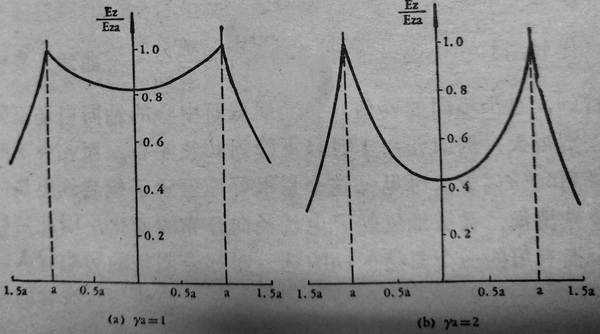
\includegraphics[width=0.65\linewidth]{figure/ch3-6}
	\caption{螺旋线中轴向电场的径向分布示意图}
	\label{ch3-6}
\end{figure}

图\ref{ch3-6}中的$ \gamma $叫做径向相位传播常数,它和$ k $、$ \beta $以下式相联系:
\begin{equation} \label{eq:3-23}
	\gamma^2 = \beta^2 - k^2
\end{equation}

将$ k= \frac{\omega}{c} $及$ \beta = \frac{\omega}{v_p} $代入\eqref{eq:3-23}式,即得:
\begin{equation} \label{eq:3-24}
	\gamma = \beta\sqrt{1 - \left( \frac{v_p}{c} \right)^2}
\end{equation}

在一般行波管中,慢波比$ \frac{v_p}{c} $都比1小很多,因此,可以认为$ \gamma \approx \beta = \frac{2\pi}{\lambda_g} $

比较图\ref{ch3-6}中$ \gamma_a = 1 $和$ \gamma_a = 2 $时的$ \frac{E_z}{E_{za}} \textasciitilde \gamma$曲线,我们可以看到,对于不同的$ \gamma_a $值,螺旋线截面中心的轴向电场下降情况差别很大,例如$ \gamma_a = 1 $时只下降到80\%左右,而$ \gamma_a = 2 $时却下降到50\%以下。可见这个量很好地表示了螺旋线电场的径向分布情况,灵敏地反映了电场径向分布的变化,因此是行波管中很有用的一个参量,$ \gamma_a $的选在1.3\textasciitilde1.6之间。
\begin{figure}[phtb]
	\centering
	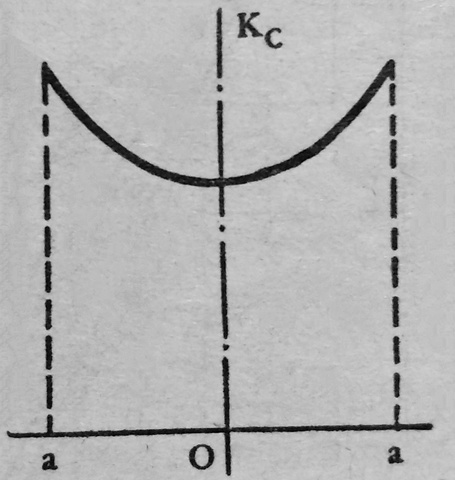
\includegraphics[width=0.3\linewidth]{figure/ch3-7}
	\caption{螺旋线耦合阻抗的径向分布}
	\label{ch3-7}
\end{figure}


为综合考虑$ \frac{b}{a} $和$ \gamma_a $对耦合阻抗的影响,通常是将理论分析的计算结果作成如图\ref{ch3-8}所示的曲线。其纵坐标为$ K_s\frac{v_p}{c} $,$ K_s $是把螺旋线简化成自由螺旋导面”(下面将介绍此模型)后得到的耦合阻抗。横坐标是$ \gamma_a $,并以$ \frac{b}{a} $为参变量作出不同$ \frac{b}{a} $值下的一组曲线。

\begin{figure}[phtb]
	\centering
	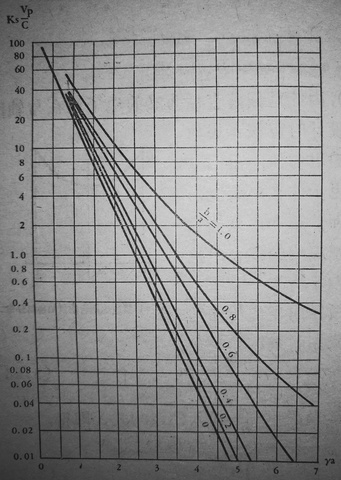
\includegraphics[width=0.5\linewidth]{figure/ch3-8}
	\caption{对于不同的$ \frac{b}{a} $螺旋线耦合阻抗与$ \gamma a $的关系}
	\label{ch3-8}
\end{figure}






\section{特性阻抗}

我们知道,任何传输线都有特性阻抗,例如常用同轴线的特性阻抗就有50欧姆和75欧姆两种。特性阻抗是传输线的一个重要参量。当两种传输线联接在一起时,为了保证传输质量我们就要求它们的特性阻抗相匹配。

慢波线也是一种传输线,它也有自己的特性阻抗,因此当它与其它传输线(如同轴线或波导)相连接时,也有匹配的问题。在设计行波管的输入输出耦合装置时就要用到特性阻抗。

慢波线特性阻抗的定义比较多,我们只介绍一种,即:
\begin{equation} \label{eq:3-25}
	Z_0 = \frac{1}{2}\frac{\hat{U_t^2}}{P}
\end{equation}
可以看出,它的形式和耦合阻抗很相似,不同的地方在于把轴向高频电压$ \hat{U_Z} $换成了横向高频电压$ \hat{U_t} $,因此$ Z_0 $又称为横向阻抗。$ \hat{U_t} $可由下式求得:
\begin{equation} \label{eq:3-26}
	\hat{U_t} = - \int_{0}^{\infty} \tilde{E_r}dr
\end{equation}
式中$ \hat{E_r} $为径向电场。若慢波线外面有金属屏蔽筒,其半径为$ c $则\eqref{eq:3-26}式变为:
\begin{equation} \label{eq:3-27}
	\hat{U_t} = -\int_{0}^{c}\tilde{E_r}dr
\end{equation}
将\eqref{eq:3-27}式代入\eqref{eq:3-25}式,即可得到慢波线的特性阻抗$ Z_0 $。特性阻抗的计算比较复杂,我们只要了解它的物理意义就行了。 

\section{实际的螺旋线}
在前面介绍螺旋线的色散特性和耦合阻抗时,我们引用了一些理论计算的结果,这些结果是在对实际的螺旋线进行了一定的简化假设以后经过适当的理论分析而得到的。这个简化假设就是把螺旋线看成所谓“自由螺旋导面”,这个螺旋导面是一个只沿螺旋方向理想导电而在其垂直方向理想绝缘的薄壁圆筒,圆筒的半径等于螺旋线的平均半径,而且处于自由空间中,即在它周围不存在任何介质及导电物体。

这个螺旋导面模型由于抓住了螺旋线的本质和特点,所以使计算结果能够比较准确地反映了它的基本特性。当然,由于模型与实物毕竞存在一定差别,为了更准确地掌握螺旋线的特性,还应该考虑某些实际因素的影响。

行波管中实际使用的螺旋线是用钼丝绕成的,像个柔软而细长的弹簧,必须用适当的方式把它夹持、固定于行波管内为了减少电磁波传播时的能量损耗,夹持另件都用高频损耗较小的介质材料如石英、纯氧化铝陶瓷、宝石等作成。为了保证螺旋线有很好的笔直度(便于电子通过)和强度,介质夹持另件常作成圆棒或条状放置在螺旋线周围。此外,为了防止电磁波向外辐射,所以螺旋线外面还有同轴放置的金属屏蔽筒(如图\ref{ch3-9})。
\begin{figure}[phtb]
	\centering
	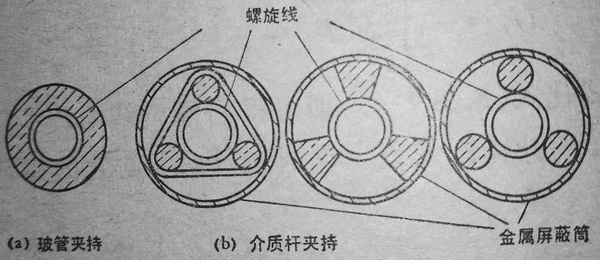
\includegraphics[width=0.65\linewidth]{figure/ch3-9}
	\caption{几种常用的螺旋线加持方法(横截面图)}
	\label{ch3-9}
\end{figure}

下面就来看看实际螺旋线中的介质、屏蔽筒及导丝对螺旋线特性的影响:
\subsection{介质夹持对色散特性的影响}
介质夹持会使相速$ v_p $下降。下降的程度用一个修正因子“DLF”来衡量。DLF的定义是:有介质夹持时的相速与无介质夹持时相速之比。所以DLF是个修正系数,因为介质的存在总是使相速下降,所以DLF必小于1。其数值大小与夹持材料的性质、夹持杆形状、尺寸等因素有关。例如几种常用夹持方式的DLF如下表:
\begin{table} 
	\caption{几种常用夹持方式的DLF}\label{tab:3-1}
	\begin{tabular}{ccccc}
		\toprule
		\centering 
		夹持方式 & 三根石英杆                  & 三根95\%Al$ _2 $O$ _3 $瓷杆 & 三根BeO瓷杆 & 嵌在玻璃管内                    \\ \midrule
		DLF                & 0.9\textasciitilde 0.95 & 0.85                    & 0.80    & 0.80\textasciitilde 0.85 \\ \bottomrule
	\end{tabular}
\end{table}


 另外,DLF还与工作频率有关。当频率很高时,$ \lambda_g $较短,场沿半径方向向外衰减很快,因此$ v_p $受介质的影响较少。而在低频端,$ \lambda_g $较长,场沿半径方向向外衰减缓慢,所以受介质影响较大,使$ v_p $下降较多。因此,介质的存在可以使色散曲线变得更加平坦,如图\ref{ch3-10}所示。这有助于增加行波管的频宽。
 \begin{figure}[phtb]
 	\centering
 	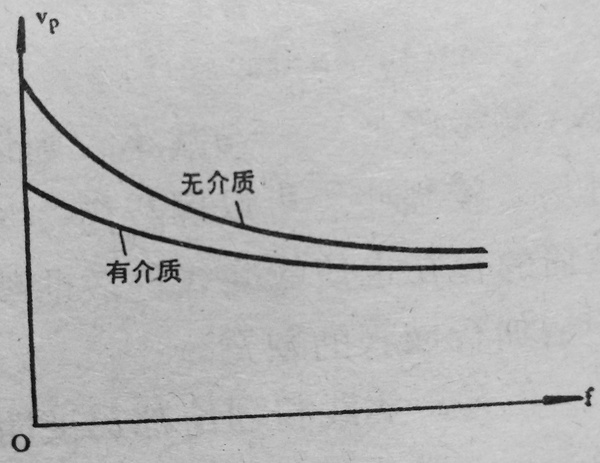
\includegraphics[width=0.45\linewidth]{figure/ch3-10}
 	\caption{介质的存在使$ v_p-f $ 曲线变得更平坦}
 	\label{ch3-10}
 \end{figure}

\subsection{屏蔽筒对色散特性的影响}
如果在“螺旋导面”模型外面再加上一个同轴放置的金属屏蔽筒(筒的半径用$ c $表示),经过理论计算,得出有屏蔽筒时的色散特性。结果表明屏蔽筒的存在也会使相速进一步降低其降低的程度也可用一个修正因子“SLF”来衡量,SLF称作屏蔽筒加载因子。计算结果如图(\ref{ch3-11})所示。
\begin{figure}[phtb]
	\centering
	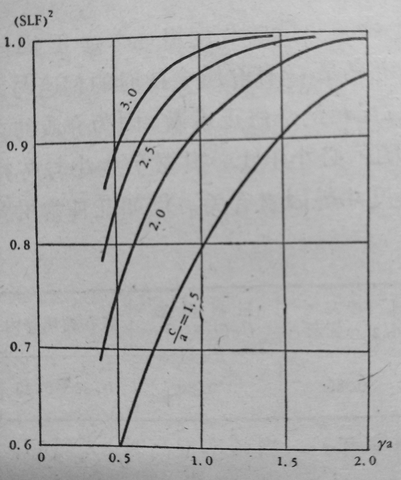
\includegraphics[width=0.48\linewidth]{figure/ch3-11}
	\caption{屏蔽筒加载因子SLF$ ^2 \textasciitilde \gamma a$曲线}
	\label{ch3-11}
\end{figure}

可以看出,$ \gamma_a $愈大,屏蔽筒的影响愈小,即SLF越接近于1。如果$ a $保持不变,那么当频率升高时,$ \gamma_a $就要增大,此时$ \lambda_g $变小,电场更加集中在“螺旋导片”附近,沿半径方向向外衰减很快,到屏蔽筒处场已很弱,所以屏蔽筒产生的相速下降较小;相反,若仍保持$ a $不变,频率降低因而$ \gamma_a $减小,则情况相反,这时$ \lambda_g $较大,屏蔽筒处场要较强些,所以屏蔽筒产生的相速下降要多些。可见,屏蔽筒的存在也使螺旋线色散曲线变得更为平坦,因而同样有助于增加行波管的频宽。

但是,实践和理论都已证明,在行波管常遇到的$ \gamma_a $范围内当$ \frac{c}{a} > 2$时,屏蔽筒对相速的影响就已小得可以忽略不计。
\subsection{介质夹持和屏蔽筒对耦合阻抗的影响}
介质夹持和屏蔽筒都使耦合阻抗降低。它们引起耦合阻抗的降低程度可以分别用介质夹持阻抗降低因子$ F_D $及屏蔽筒阻抗降低因子$ F_s $来修正,它们都是小于1的数。而且当$ \frac{c}{a} > 2$时,$ F_s $接近于1,这时$ F_s $的影响可以忽略不计。$ F_D $在一般常遇到的条件下大约为0.6\textasciitilde0.8。$ F_D $和DLF之间的关系可从曲线查到。
\subsection{导丝尺寸的影响}
由于实际的螺旋线是由金属导丝绕成的,并不是理想的螺旋导片,因而并不是一个均匀慢波线,也会引起耦合阻抗下降,为此,也引入一个阻抗降低因子$ F_\delta $,一般$ F_\delta $在0.7\textasciitilde0.9之间。

因此,一个实际螺旋线的耦合阻抗$ K_c $应为
\begin{equation} \label{eq:3-28}
	K_c = K_s \cdot F_s \cdot F_\delta
\end{equation}

式中$ K_s $为自由空间里螺旋导面的耦合阻抗。通常$ K_c $的数值在20\textasciitilde100欧姆之间。















